\begin{pastexam}[label={px:df3-104-ds-04}]{地方三等資訊處理 104 年 第四題}
（申論；20 分）

\begin{itemize}[leftmargin=2em, labelsep=0.3em, itemsep=2pt]
\item[㈠] 一運算式（expression）為：$-a+(z+f)/y-b*a/c+d$，請依運算元優先順序，繪出其二元樹
（binary tree）。（10 分）
\item[㈡] 請列出此二元樹的前序走訪（preorder traversal）。（5 分）
\item[㈢] 請列出此二元樹的廣度優先走訪（breadth-first search traversal）。（5 分）
\end{itemize}
\end{pastexam}

\begin{pastsoln}
題目的「運算元優先順序」指的是運算子（operator）的優先順序，照一般算術規則：括號最優先，
其次是開頭的\textbf{負號}（一元運算子，只有一個運算元），再來是 $*$、$/$，最後是 $+$、$-$；
同一級由左到右結合。 下面把負號畫成只有一個子節點的節點，在走訪結果裡寫成 $\ominus$，和減號
$-$ 區分。 （若把 $-a$ 看成 $0 - a$，就是把 $\ominus$ 節點換成左子 $0$、右子 $a$ 的減號節點，
其餘不變。）

\textbf{㈠} 先加上括號標出計算順序：
\[
\Bigl(\bigl(\,(\ominus a) + ((z + f) / y)\,\bigr) - ((b * a) / c)\Bigr) + d .
\]
最後才做的運算是最右邊那個 $+$（$+$、$-$ 同級，由左到右結合，最右邊的最後做），它是根；左運算元是
$(\ominus a) + (z+f)/y - b*a/c$，右運算元是 $d$。 左邊再拆：最後做的是 $-$，左邊
$(\ominus a) + (z+f)/y$、右邊 $b*a/c$；依此類推（資結書第~7.7~節）。
\begin{center}
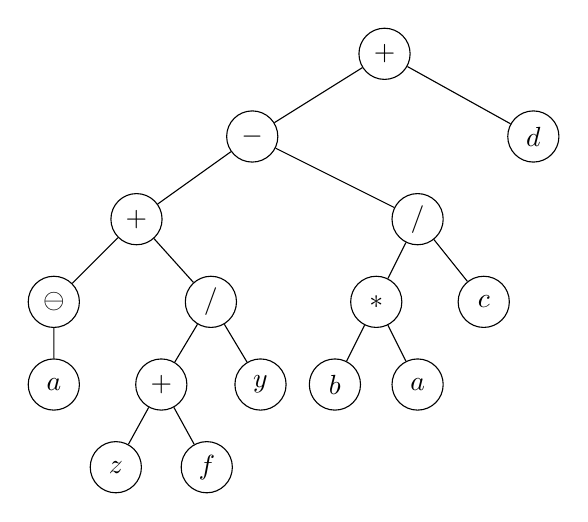
\begin{tikzpicture}[x=1.05cm, y=1.05cm,
  n/.style={circle, draw, minimum size=6.5mm, inner sep=0pt}]
\node[n] (r) at (4,0) {$+$};
\node[n] (m) at (2.4,-1) {$-$};
\node[n] (d) at (5.8,-1) {$d$};
\node[n] (p) at (1,-2) {$+$};
\node[n] (q) at (4.4,-2) {$/$};
\node[n] (u) at (0,-3) {$\ominus$};
\node[n] (s) at (1.9,-3) {$/$};
\node[n] (t) at (3.9,-3) {$*$};
\node[n] (c) at (5.2,-3) {$c$};
\node[n] (a1) at (0,-4) {$a$};
\node[n] (zf) at (1.3,-4) {$+$};
\node[n] (y) at (2.5,-4) {$y$};
\node[n] (b) at (3.4,-4) {$b$};
\node[n] (a2) at (4.4,-4) {$a$};
\node[n] (z) at (0.75,-5) {$z$};
\node[n] (f) at (1.85,-5) {$f$};
\draw (r)--(m) (r)--(d) (m)--(p) (m)--(q) (p)--(u) (p)--(s) (q)--(t) (q)--(c)
      (u)--(a1) (s)--(zf) (s)--(y) (t)--(b) (t)--(a2) (zf)--(z) (zf)--(f);
\end{tikzpicture}
\end{center}
檢查：中序走訪（加回括號）是 $(((\ominus a) + ((z+f)/y)) - ((b*a)/c)) + d$，和原式相同；
$\ominus$ 只有一個子節點，其他運算子節點都有兩個，葉節點都是運算元。

\textbf{㈡ 前序走訪}（根、左、右）：
\[
+ \;\; - \;\; + \;\; \ominus \;\; a \;\; / \;\; + \;\; z \;\; f \;\; y \;\; / \;\; * \;\; b \;\; a \;\; c \;\; d
\]
也就是運算式的前序式 $+\,-\,+\,\ominus\,a\,/\,+\,z\,f\,y\,/\,*\,b\,a\,c\,d$。

\textbf{㈢ 廣度優先走訪}（一層一層、每層由左到右，資結書第~7.3.2~節）：
\begin{center}
\begin{tabular}{cl}
\toprule
層 & 節點 \\
\midrule
0 & $+$ \\
1 & $-$,\ $d$ \\
2 & $+$,\ $/$ \\
3 & $\ominus$,\ $/$,\ $*$,\ $c$ \\
4 & $a$,\ $+$,\ $y$,\ $b$,\ $a$ \\
5 & $z$,\ $f$ \\
\bottomrule
\end{tabular}
\end{center}
所以廣度優先走訪的順序是
\[
+ \;\; - \;\; d \;\; + \;\; / \;\; \ominus \;\; / \;\; * \;\; c \;\; a \;\; + \;\; y \;\; b \;\; a \;\; z \;\; f .
\]
\end{pastsoln}
